\chapter{Configurazione}
\label{Configurazione}
\thispagestyle{empty}

\section{Primo avvio}
Una volta eseguito Docker Compose, il sistema risulta avviato, funzionante e raggiungibile sulla porta 80, dall'host all'indirizzo \verb|localhost|, oppure da una macchina collegata alla rete locale tramite \verb|hostname|. Per quanto riguarda l'installazione fatta in ateneo, la macchine è raggiungibile all'indirizzo \verb|sharelatex.ing.unimore.it|, che verrà preso come esempio per i passi futuri.

Per prima cosa è necessario registrare l'amministratore del sistema all'indirizzo\\\verb|sharelatex.ing.unimore.it/launchpad|. Una volta inseriti indirizzo e-mail e password dell'amministratore, verrà richiesto il primo login. Inserite le credenziali dell'amministratore, verrà mostrata il launchpad, il quale mostra lo stato dell'editor e delle websocket e dal quale è possibile inviare un'email di test a un indirizzo a scelta\footnote{Per usufruire di questa funzionalità è necessario configurare il servizio mail con \hyperref[SMTP]{SMTP}.}
\begin{figure}[h]
    \begin{subfigure}{0.5\textwidth}
        \centering
        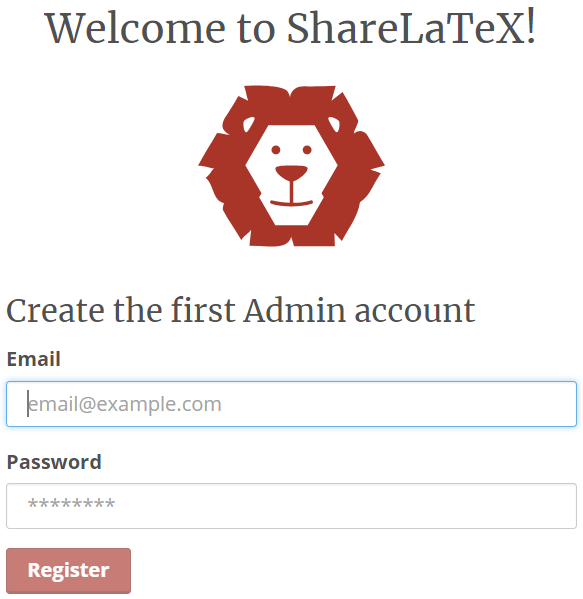
\includegraphics[height=7cm]{immagini/launchpad_1.png}
        \caption{Launchpad}
        \label{fig:sharelatex_launchpad_1}
    \end{subfigure}
    \begin{subfigure}{0.5\textwidth}
        \centering
        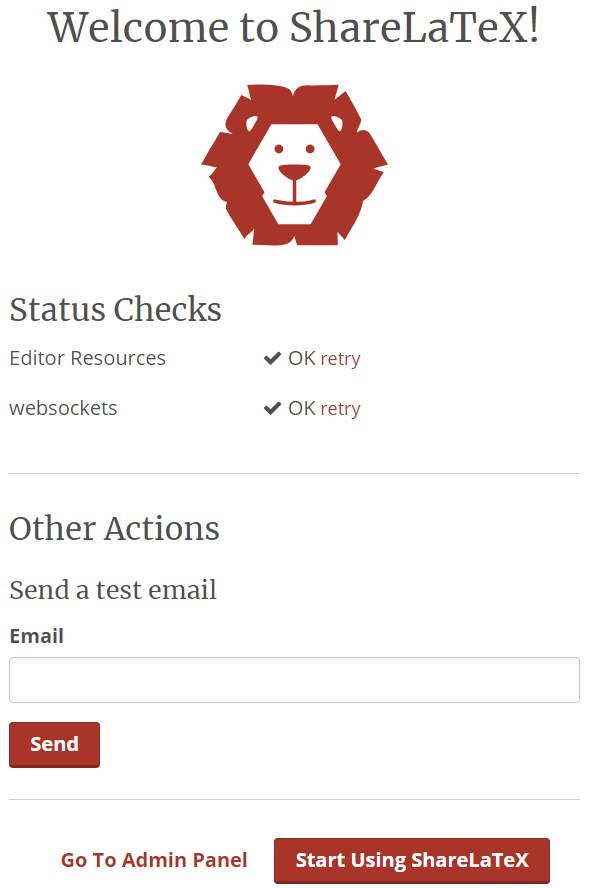
\includegraphics[height=7cm]{immagini/launchpad_2.png}
        \caption{Schermata di controllo}
        \label{fig:sharelatex_launchpad_2}
    \end{subfigure}
    \caption{Creazione utente amministratore}
    \label{fig:sharelatex_launchpad}
\end{figure}


\section{Interfaccia}
\verb|docker-compose.yml| permette di impostare variabili d'ambiente all'interno dei container. ShareLaTeX è altamente configurabile sotto questo aspetto. Si elencano le variabili d'ambiente utilizzate per l'installazione in ateneo.
\begin{itemize}
    \item \verb|SHARELATEX_APP_NAME|: nome dell'applicazione, che sarà mostrato nella barra di navigazione del browser.
    \item \verb|SHARELATEX_NAV_TITLE|: nome dell'applicazione, che sarà mostrato in alto a sinistra nell'homepage del profilo utente.
    \item \verb|SHARELATEX_HEADER_IMAGE|: URL di un'immagine, che sarà mostrata in alto a sinistra. Nel caso in cui \verb|SHARELATEX_NAV_TITLE| fosse impostato, allora\\\verb|SHARELATEX_HEADER_IMAGE| avrà la priorità.
    \item \verb|SHARELATEX_SITE_URL|: indirizzo della macchina host del servizio.
    \item \verb|SHARELATEX_ADMIN_EMAIL|: indirizzo e-mail dell'amministratore di sistema, che sarà mostrata in fase di registrazione utente.
    \item \verb|SHARELATEX_LEFT_FOOTER|: array JSON in cui si può aggiungere testo HTML che verrà mostrato in basso a sinistra nell'homepage.
    \item \verb|SHARELATEX_RIGHT_FOOTER|: array JSON in cui si può aggiungere testo HTML che verrà mostrato in basso a destra nell'homepage.
    \item \verb|SHARELATEX_SITE_LANGUAGE|: lingua dell'applicazione. Di default la lingua impostata è inglese, ma sono disponibili anche:
        \begin{multicols}{3}
            \begin{itemize}
                \item es = spagnolo
                \item pt = portoghese
                \item de = tedesco
                \item fr = francese
                \item cs = ceco
                \item nl = olandese
                \item sv = svedese
                \item it = italiano
                \item tr = turco
                \item cn = cinese
                \item no = norvegese
                \item da = danese
                \item ru = russo
                \item ko = coreano
                \item ja = giapponese
            \end{itemize}
        \end{multicols}
\end{itemize}

\section{Registrazione utenti e SMTP}
\label{SMTP}
L'amministratore può registrare utenti normali all'applicazione aggiungendo la loro email nella pagina "Manage Users". La piattaforma genera un link per impostare la password del nuovo account. Questo link deve essere in qualche modo consegnato al nuovo utente. Se il servizio email è configurato, allora questa fase sarà automatica. I parametri sono passati mediante variabili d'ambiente. Si raccomanda impostare \verb|SHARELATEX_SITE_URL| per generare link di iscrizione funzionanti. Si elencano le variabili d'ambiente utilizzate per l'installazione in ateneo.
\begin{itemize}
    \item \verb|SHARELATEX_EMAIL_FROM_ADDRESS|: indirizzo del mittente del messaggio.
    \item \verb|SHARELATEX_EMAIL_SMTP_HOST|: host del servizio SMTP.
    \item \verb|SHARELATEX_EMAIL_SMTP_PORT|: porta SMTP da utilizzare.
    \item \verb|SHARELATEX_EMAIL_SMTP_SECURE|: valore booleano che, se vero, attiva SMTPS.
    \item \verb|SHARELATEX_EMAIL_SMTP_USER|: nome utente da autenticare.
    \item \verb|SHARELATEX_EMAIL_STMP_PASS|: password dell'utente da autenticare.
    \item \verb|SHARELATEX_EMAIL_STMP_TLS_REJECT_UNAUTH|: valore booleano che, se vero, rifiuta connessioni TLS (Transport Layer Security) non autorizzate.
    \item \verb|SHARELATEX_EMAIL_STMP_IGNORE_TLS|: valore booleano che, se vero, disattiva il supporto STARTTLS.
    \item \verb|SHARELATEX_CUSTOM_EMAIL_FOOTER|: testo HTML con cui si può personalizzare il footer delle email.
\end{itemize}